\documentclass[11pt]{article}
\usepackage[a4paper,margin=0mm]{geometry}
\usepackage{fontspec}
\usepackage[french]{babel}
\usepackage{xcolor}
\usepackage{tikz}
\usepackage[most]{tcolorbox}
\usepackage{pdfpages}
\usepackage{hyperref}
\setmainfont{DejaVu Serif}
\setsansfont{DejaVu Sans}
\definecolor{EDBlue}{HTML}{214D6B}
\definecolor{EDGold}{HTML}{F7F1DE}
\definecolor{EDGreen}{HTML}{EDF5EA}
\definecolor{EDPaleBlue}{HTML}{EAF2F7}
\definecolor{EDGrey}{HTML}{6F6F6F}
\pagestyle{empty}

\hypersetup{
  pdftitle={ED-POMDP - De la croyance à l'action - Companion FR v1.0},
  pdfauthor={Guillaume Harbonnier},
  pdfsubject={Export autonome de l'ancienne Annexe G du guide v1.8}
}
\begin{document}
\null
\begin{tikzpicture}[remember picture,overlay]
  \node[anchor=north east,text=EDGrey,font=\fontsize{8.5}{10}\selectfont] at ([xshift=-28mm,yshift=-9mm]current page.north east) {ED-POMDP - Document companion avancé};
  \node[anchor=north,text=EDBlue,font=\bfseries\fontsize{25}{30}\selectfont] at ([yshift=-58mm]current page.north) {ED-POMDP};
  \node[anchor=north,text=EDBlue,font=\bfseries\fontsize{19}{23}\selectfont] at ([yshift=-78mm]current page.north) {DE LA CROYANCE À L'ACTION};
  \node[anchor=north,font=\fontsize{12}{15}\selectfont] at ([yshift=-96mm]current page.north) {Estimation d'état, recherche opérationnelle et apprentissage de politiques};
  \node[anchor=north,fill=EDGold,rounded corners=5mm,text width=126mm,inner xsep=7mm,inner ysep=7mm,align=justify,font=\fontsize{10.2}{11.5}\selectfont] at ([yshift=-131mm]current page.north) {Document autonome de niveau avancé. Il reproduit sans modification scientifique l'ancienne Annexe G du guide ED-POMDP en clair v1.8. Les deux pages liminaires ajoutent seulement le contrat de lecture, les prérequis et des repères terminologiques.};
  \node[anchor=north west,text=EDBlue,font=\bfseries\fontsize{13}{15}\selectfont] at ([xshift=35mm,yshift=-194mm]current page.north west) {Prérequis conseillés};
  \node[anchor=north west,text width=140mm,align=left,font=\fontsize{10.2}{11.5}\selectfont] at ([xshift=35mm,yshift=-207mm]current page.north west) {Probabilités conditionnelles, espérance, mise à jour bayésienne, optimisation, notions de machine learning et lecture générale d'un MDP/POMDP.};
  \node[anchor=south,text=EDGrey,font=\fontsize{9}{10}\selectfont] at ([yshift=18mm]current page.south) {Companion français uniquement - Version 1.0};
\end{tikzpicture}
\newpage

\null
\begin{tikzpicture}[remember picture,overlay]
  \node[anchor=north east,text=EDGrey,font=\fontsize{8.5}{10}\selectfont] at ([xshift=-28mm,yshift=-9mm]current page.north east) {ED-POMDP - Document companion avancé};
  \node[anchor=north west,text=EDBlue,font=\bfseries\fontsize{20}{24}\selectfont] at ([xshift=25mm,yshift=-27mm]current page.north west) {Repères terminologiques du companion};
  \node[anchor=north west,text width=160mm,align=justify,font=\fontsize{10}{11.5}\selectfont] at ([xshift=25mm,yshift=-48mm]current page.north west) {Les familles d'estimateurs citées sont un panorama de choix possibles, pas un cours complet. Le texte conserve certains noms anglais lorsqu'ils correspondent aux termes canoniques de la littérature.};
  \foreach \x/\y/\bg/\title/\body in {
    25/86/EDGreen/{MAP}/{Maximum a posteriori : état le plus probable après observation.},
    25/117/EDPaleBlue/{Marginalisation}/{Sommer ou intégrer les autres variables pour ne garder que la distribution d'intérêt.},
    25/148/EDGreen/{HMM}/{Modèle de Markov caché : état latent évolutif observé indirectement.},
    25/179/EDPaleBlue/{Filtre de Kalman}/{Estimateur récursif pour un modèle linéaire gaussien.},
    25/210/EDGreen/{Filtre particulaire / SMC}/{Approximation d'une distribution par un ensemble de particules pondérées.},
    25/241/EDPaleBlue/{Inférence amortie}/{Modèle appris qui produit rapidement une approximation de la croyance.},
    110/86/EDGreen/{Ensemble conforme}/{Ensemble de prédictions muni d'une garantie de couverture sous hypothèses données.},
    110/117/EDPaleBlue/{Bandit contextuel}/{Choix répété d'une action à partir d'un contexte, sans modèle d'état complet.},
    110/148/EDGreen/{RL model-based}/{Apprentissage ou planification avec un modèle explicite des transitions.},
    110/179/EDPaleBlue/{RL model-free}/{Apprentissage direct d'une valeur ou politique sans modèle explicite complet.},
    110/210/EDGreen/{Offline RL}/{Apprentissage d'une politique à partir de données historiques, sans exploration en ligne.},
    110/241/EDPaleBlue/{Contrainte dure}/{Condition qui ne peut pas être compensée par un gain sur un autre objectif.}
  }{
    \node[anchor=north west,fill=\bg,rounded corners=3mm,minimum width=77mm,minimum height=25mm,text width=69mm,inner xsep=4mm,inner ysep=3mm,align=left] at ([xshift=\x mm,yshift=-\y mm]current page.north west) {\textcolor{EDBlue}{\bfseries\fontsize{8.2}{9}\selectfont \title}\\[0.4mm]{\fontsize{7.1}{8.1}\selectfont \body}};
  }
  \node[anchor=south,text=EDGrey,font=\fontsize{8.5}{10}\selectfont] at ([yshift=14mm]current page.south) {Les sept pages suivantes sont reprises à l'identique de l'Annexe G de la v1.8.};
\end{tikzpicture}
\newpage

\includepdf[pages=31-37,fitpaper=true,pagecommand={}]{base/ED_POMDP_En_Clair_FR_v1.8.pdf}
\end{document}
